\section{Shor's Algorithmus}\newline

	Kryptografische Systeme basieren heutzutage oft auf dem Prinzip des RSA-Algorithmus. Durch eine mathematische \textit{Falltür} kann RSA nur in eine Richtung, in diesem Fall die Verschlüsselung, berechnet werden. Die andere Richtung ist die Entschlüsselung, deren Berechnung ohne Kenntnis des Schlüssels je nach Schlüsselgröße mit heutigen Supercomputern mehrere Menschenleben lang dauert. 


	Diese \textit{Falltür} besteht grundlegend aus dem Faktorisieren des Produkts zweier großer Primzahlen. Die Berechnung der Faktoren dauert mit aktuell anwendbaren Algorithmen eine \textit{superpolynome} Zeit lang.
	Shor's Algorithmus faktorisiert das Produkt von zwei Primzahlen in nur \textit{polynomer} Zeit, was signifikant schneller ist und somit das Falltürprinzip von RSA in Frage stellt.
	\newline\newline
    

	\hr
    \textbf{Einschub:}

   
        Primzahlen sind natürliche Zahlen und nur durch sich selbst und 1 teilbar. Ein Beispiel für Primzahlen sind 3 oder 5. Das Gesetz der Primfaktorzerlegung besagt, dass jede natürliche Zahl, die keine Primzahl ist, sich als Produkt von mindestens zwei Primzahlen schreiben lässt. So lässt sich die natürliche Zahl 15, die keine Primzahl ist, beispielsweise auch als \(3\cdot 5\) schreiben.
   \newline 
   \hr
	\newline

	Der Shor Algorithmus macht Gebrauch davon, ein Problem in ein anderes zu transformieren, dessen Lösung simpler ist. \glqq Anstatt einen Quantencomputer-Algorithmus für die direkte Faktorisierung von n zu erstellen, verwenden wir einen Quantencomputer-Algorithmus zur Bestimmung der Ordnung eines Elements \(a\) in der multiplikativen Gruppe \(\pmod{n}\), d.h. die kleinste ganze Zahl \(r\), bei der \(a^r \equiv 1 \pmod{n} \) ist. [Durch Miller] ist bekannt, dass die Faktorisierung mit Hilfe von Zufallszahlen auf die Suche nach der Reihenfolge eines Elements reduziert werden kann.\grqq (Shor, 1997, S. 15) (Miller, 1976, Vgl.) Das Faktorisierungsproblem wird also zu einem periodischen Problem transformiert.

	\begin{figure}
        \centering
        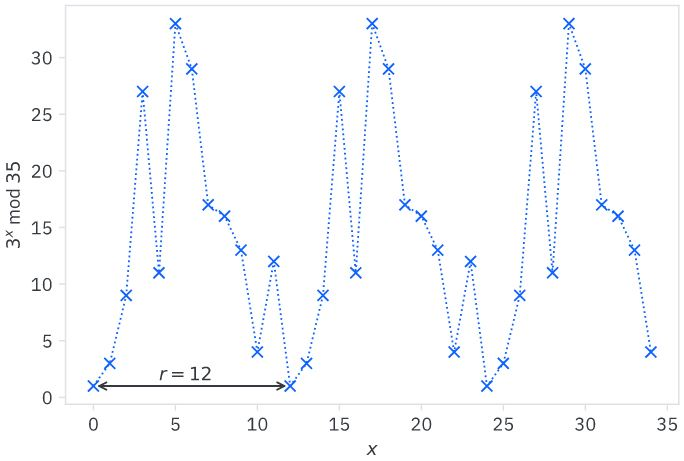
\includegraphics[width=9cm]{content/periodicExample.JPG}
        \caption{Beispiel der periodischen Funktion \(f(x) = a^x\bmod{n}\) aus Shor's Algorithmus mit \(a=3\), \(n=35\) und der Ordnung \(r=12\). (ANIS u. a., 2021, Textbook ’Shor’s
        Algorithm’ - Chapter 1)}
        \label{fig:periodicExample}
    \end{figure}

	\newline
		\exercise[type=multipleChoice]{
			\question{
					Frage: Zu welchem Problem wird das Faktorisierungsproblem umgewandelt?
			}
			\possibleAnswers{
					\item 1) Zu einem Falltürproblem.
					\item 2) Zu einem periodischen Problem.
					\item 3) Zu einer Quantenschaltung.
			}
			\result{2}
	}
	\newline \newline

	Eine periodische Funktion mit Shor's genannten Bedingungen lässt sich mit den natürlichen Zahlen \(a\), die eine Zufallszahl ist, und dem zu faktorisierenden Produkt \(n\) mit \(a < n\) wie folgt definieren:

	\begin{equation}
	    f(x) = a^x\bmod{n}.
		\quad \quad (1)
	\end{equation}

	\newline

    Diese periodische Funktion besitzt eine Ordnung \(r\) (Länge einer Periode), die für das Lösen des Faktorisierungsproblems benötigt wird und ist die kleinstmögliche natürliche Zahl für die gilt:

	\begin{equation}\begin{aligned}\label{eq:17}
	    a^r\bmod{n} &= 1 \\
	    (a^r-1)\bmod{n} &= 0.
	    \end{aligned}
    \quad \quad (2)
	\end{equation}


    Nachdem die Ordnung \(r\) mithilfe des Quanten-Algorithmus berechnet wurde, folgt die Umformung des nun gelösten Periodenproblems zurück in ein Faktorisierungsproblem. 
    Falls \(r\) nicht gerade ist, muss eine andere zufällige Zahl \(a\) gewählt werden, da folgende Umformung sonst nicht möglich ist:
    \begin{equation} \label{eq:shorUmformung}
         a^r-1 = (a^\frac{r}{2}-1)(a^\frac{r}{2}+1).  
		 \quad \quad (3)
    \end{equation}

	Die Umformung wird mit der Erkenntnis aus dem zweiten Teil von Gleichung (2) durchgeführt, dass \(n\) ein Teiler von \(a^r-1\) sein muss.  (ANIS u. a., 2021, Vgl. Textbook ’Shor’s Algorithm’ - Chapter 5)  Es besteht die Wahrscheinlichkeit \(P_{min}=1-\frac{1}{2^{k-1}}\) mit \(k\) als Anzahl der ungeraden Primfaktoren von \(n\), dass der größte gemeinsame Teiler \(ggT\begin{pmatrix}a^\frac{r}{2}-1; n\end{pmatrix}\) ein Faktor von \(n\) ist. (Shor, 1997, Vgl. S. 15-16) Der größte gemeinsame Teiler kann mithilfe des euklidischen Algorithmus effizient berechnet werden.\newline

	Der \textbf{Quanten-Algorithmus} zur Berechnung der Ordnung \(r\) verwendet \textit{Quantum Phase Estimation} zusammen mit dem unitären Operator \textit{U}. Die periodische Funktion aus Formel (1) wird wie folgt umgebaut:

	\begin{equation}\label{eq:19}
	    U \Ket{y} \equiv \Ket{a y \bmod{n}}.  \quad \quad (4)

	\end{equation}
	Jede Anwendung von \textit{U} multipliziert den Zustand des Registers \(\Ket{y}\) mit \(a\pmod{n}\). Beginnt \(\Ket{y}\) also im Zustand \(\Ket{1}\) wird nach \textit{r} Anwendungen von \textit{U} der Zustand \(\Ket{1}\) erneut erreicht. Die Anwendung des Prinzips aus Formel (4) auf das Beispiel aus dem oberen Bild mit \(a=3\), \(n=35\) und \(r=12\)  veranschaulicht das:
	\begin{gather*}
	    U \Ket{1} = \Ket{3}, \quad U^2 \Ket{1} = \Ket{9}, \quad U^3 \Ket{1} = \Ket{27} \quad ... \quad U^{r-1} \Ket{1} = \Ket{12}, \quad U^r \Ket{1} = \Ket{1}.  \quad \quad (5)
	\end{gather*}

	Hierbei ist im Vergleich mit der Abbildung die x-Achse die Anzahl an Anwendungen von \textit{U} und die y-Achse der Zustand des Registers \(\Ket{y}\). (ANIS u. a., 2021, Vgl. Textbook ’Shor’s Algorithm’ - Chapter 2) \newline
	
	\newline \newline
	\exercise[type=multipleChoice]{
		\question{
				Frage: Was macht der unitäre Operator U in diesem Fall?
		}
		\possibleAnswers{
				\item 1) Er definiert die Zufallszahl \(a\).
				\item 2) Er führt einen Schritt in der Periode durch.
				\item 3) Er berechnet die oben genannten Primzahlen.
		}
		\result{2}
}
\newline \newline

	Um die Ordnung mithilfe von QPE zu messen, muss \(r\) als Phase vorhanden sein. Hierfür wird das Register \(\Ket{y}\) zunächst in die Superposition \(\Ket{u_0}\) gebracht, was ein valider Eigenzustand von \textit{U} ist:

	\begin{gather*}
	    \Ket{u_0} = \frac{1}{\sqrt{r}} \sum_{k=0}^{r-1} \Ket{a^k \bmod{n}} .  \quad \quad (6)
	\end{gather*}

	Das Beispiel mit \(a=3\), \(n=35\) und \(r=12\) sieht unter diesen Umständen wie folgt aus:

	\begin{align*}
	    \Ket{u_0} &= \frac{1}{\sqrt{12}} \begin{pmatrix}\Ket{1} + \Ket{3} + \Ket{9} ... \Ket{4} + \Ket{12}\end{pmatrix} \\
	    U\Ket{u_0} &= \frac{1}{\sqrt{12}} \begin{pmatrix}\Ket{3} + \Ket{9} + \Ket{27} ... \Ket{12} + \Ket{1}\end{pmatrix} = \Ket{u_0}.  \quad \quad (7)
	\end{align*}


	Dieser Eigenzustand hat einen Eigenwert von 1 und hat in diesem Kontext keine große Relevanz. \glqq Ein interessanterer Eigenzustand könnte einer sein, bei dem die Phase für jeden dieser Zustände in der Berechnungsbasis [z-Basis] unterschiedlich ist. \grqq  (ANIS u. a., 2021, Vgl. Textbook ’Shor’s Algorithm’ - Chapter 2) Wenn die Phase des \textit{k-ten} Zustands proportional zu \textit{k} ist, resultiert dies in:

	\begin{align*}
	    \Ket{u_1} &= \frac{1}{\sqrt{r}} \sum_{k=0}^{r-1} \exp{(-\frac{2\pi i k}{r})} \Ket{a^k \bmod{n}}, \\
	    U\Ket{u_1} &= \exp{(-\frac{2\pi i}{r})}  \Ket{u1}.  \quad \quad \quad \quad \quad \quad \quad \quad (8)
	\end{align*}

    Der Eigenwert beinhaltet in diesem Fall \textit{r}, was für die Überpüfung der Gleichheit der Phasendifferenzen zwischen den Zuständen der Berechnungsbasen notwendig ist. \newline
    Wird dieses Prinzip weiter ausgenutzt, so kann eine weitere ganze Zahl \textit{s} mit dieser Phasendifferenz multipliziert werden:

	\begin{align*}
	    \Ket{u_s} &= \frac{1}{\sqrt{r}} \sum_{k=0}^{r-1} \exp{(-\frac{2\pi i s k}{r})} \Ket{a^k \bmod{n}}, \\
	    U\Ket{u_s} &= \exp{(-\frac{2\pi i s}{r})}  \Ket{u1}     \quad \quad \quad \quad \quad \quad \quad \quad \quad \quad \quad \quad \quad \quad (9)
	\end{align*}


	Mit dem Beispiel \(a=3\), \(n=35\) und \(r=12\) wird daraus also:
	\begin{align*}
	    \Ket{u_s} &= \frac{1}{\sqrt{12}} \bigg( \exp{(-\frac{0\cdot 2\pi is}{12})}\Ket{1} + \exp{(-\frac{1\cdot 2\pi is}{12})}\Ket{3} \quad ... \quad \exp{(-\frac{11\cdot 2\pi is}{r})}\Ket{12} \bigg) \\
	    U\Ket{u_s} &= \frac{1}{\sqrt{12}} \bigg(\exp{(-\frac{0\cdot 2\pi is}{12})}\Ket{3} + \exp{(-\frac{1\cdot 2\pi is}{12})}\Ket{9} \quad ... \quad \exp{(-\frac{11\cdot 2\pi is}{r})}\Ket{1}\bigg) \\
	    U \Ket{u_s} &= \exp{(-\frac{2\pi i s}{12})}\Ket{u_s}  \quad \quad \quad \quad \quad \quad  \quad \quad \quad \quad \quad \quad  \quad \quad \quad \quad \quad \quad (10)
	\end{align*}


    Dadurch entstehen singuläre Eigenzustände für jeden ganzzahligen Wert von \textit{s} mit der Bedingung \(0 \leq s \leq r-1\). Durch die Aufsummierung all dieser Eigenzustände werden durch die verschiedenen Phasen alle Zustände der Berechnungsbasis bis auf \(\Ket{1}\) aufgehoben:


	\begin{align*}
	    \Ket{1} &= \frac{1}{\sqrt{r}} \sum_{s=0}^{r-1} \Ket{u_s}.  \quad \quad (11)
	\end{align*}

    Der Zustand \(\Ket{1}\) ist eine Überlagerung all dieser Eigenzustände. Die Phase des Zustands kann mit einer QPE gemessen werden:


	\begin{align*}
	    \phi = \frac{s}{r}  \quad \quad (12)
	\end{align*}

    In diesem Fall ist \textit{s} eine zufällige ganze Zahl zwischen \(0\) und \(r-1\). \newline
    \glqq Durch die Anwendung des Kettenbruch Algorithmus, [also der Approximation durch einen Näherungsbruch], auf \(\phi\), kann \(r\) berechnet werden.\grqq (ANIS u. a., 2021, Vgl. Textbook ’Shor’s Algorithm’ - Chapter 2)

    \begin{figure}
        \centering
        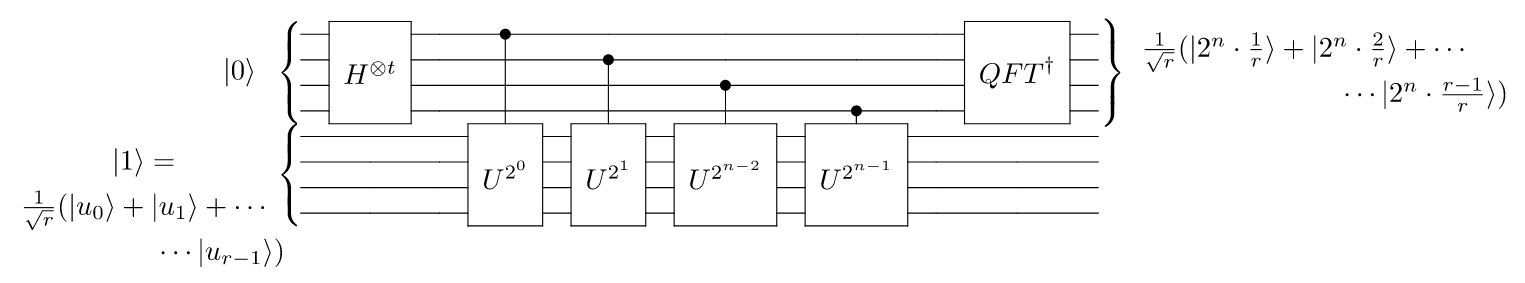
\includegraphics[width=100]{content/shor_circuit_1.JPG}
        \caption{Circuit einer Shor Algorithmus Implementation (nach der Qiskit Qubit Ordering Convention) (ANIS u. a., 2021, Vgl. Textbook ’Shor’s Algorithm’ - Chapter 2)}
        \label{fig:periodicExample}
    \end{figure}

	Die U-Gates der QPE sind in diesem Fall die dynamischen Modulo Funktionen. Jedes U-Gate führt wie in Formel (4) beschrieben eine kontrollierte Multiplikation auf die Phase von \(\Ket{y}\) mit dem Ergebnis von \(a^{2^j}\bmod{n}\) durch, wobei \(j\) die Anzahl der bereits angewendeten U-Gates ist. Mithilfe des \textit{Repeated Squaring} Algorithmus kann \(a^{2^j}\bmod{n}\) effizient berechnet werden. 
	Soll zum \textbf{Beispiel} die Zahl \(n=15\) faktorisiert werden, die das Produkt der Primzahlen \(3\) und \(5\) ist, wird wie folgt vorgegangen:

	\list{
	\item Überprüfen, ob \(n\) eine gerade Zahl ist. Wenn ja, wird der Prozess beendet und Faktor \(2\) zurückgegeben. Da \(n=15\) ungerade ist, beginnt Schritt 2.
	\item Es muss eine zufällige Zahl zwischen \(1\) und \(n-1=14\) ausgewählt werden. In diesem Beispiel wird zufällig \(a=7\) gewählt, was kein Faktor von \(n\) ist. 
	\item Mithilfe des Quanten-Algorithmus wird die Ordnung \(r\) von \(7^{r}\bmod{15}=1\) bestimmt. Wie in der letzten Abbildung erkennbar ist, weisen zwei der vier Messergebnisse auf die korrekte Ordnung \(r=4\) hin:}

	
	    \begin{figure}
            \centering
            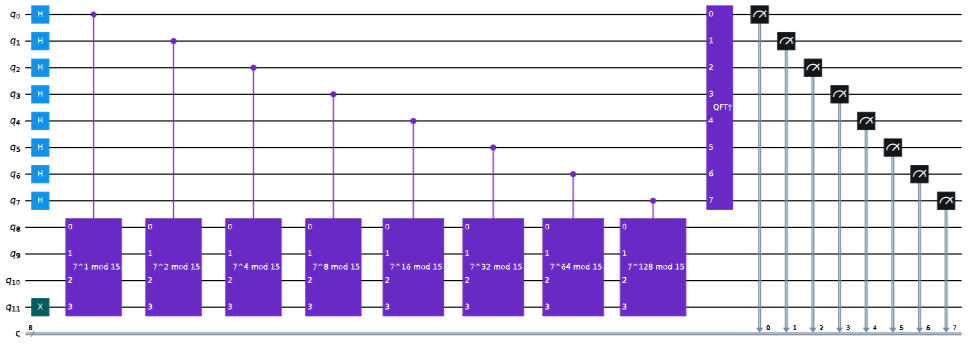
\includegraphics[width=100]{content/shor_example.PNG}
            \caption{Beispiel des Shor Algorithmus mit 8 Zählerqubits, \(n=15\) und \(a=7\) (ANIS u. a., 2021, Vgl. Textbook ’Shor’s Algorithm’ - Chapter 3)}
            \label{fig:shorExample}
        \end{figure}

        \begin{figure}
            \centering
            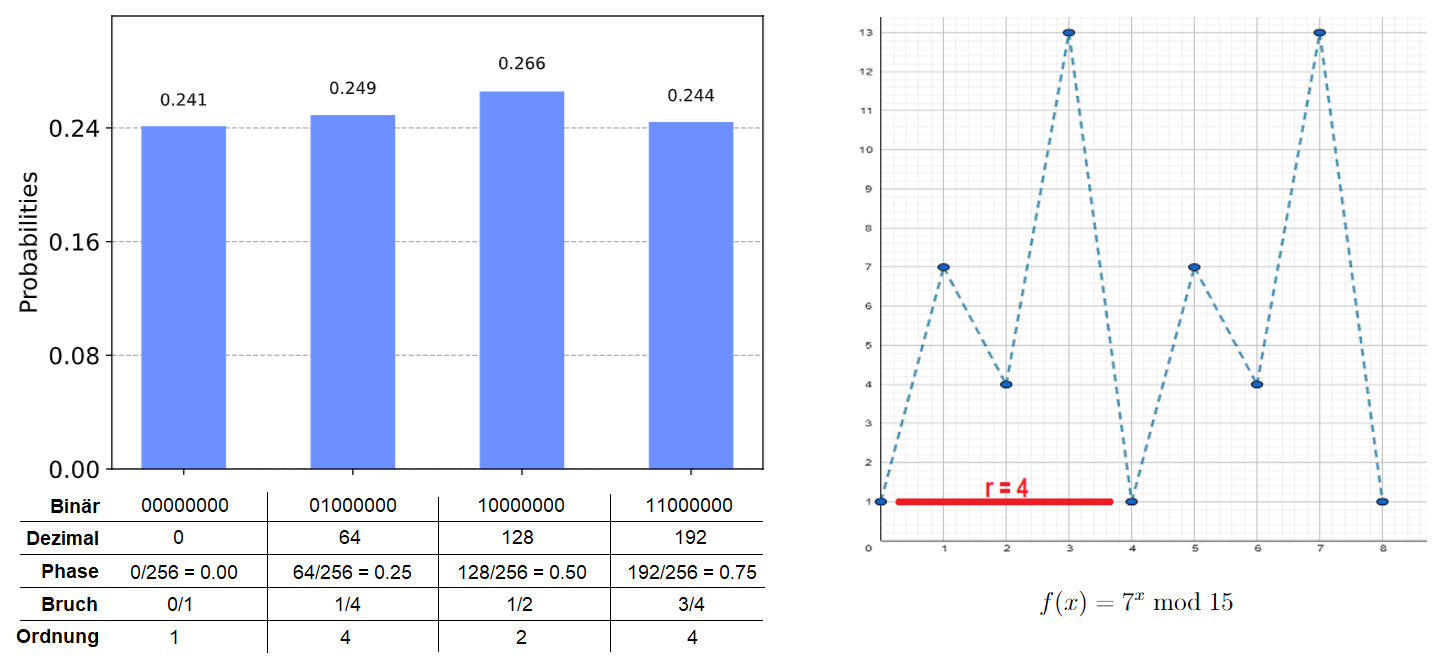
\includegraphics[width=100]{content/shor_beispiel_messung.png}
            \caption{Durchschnittliches Messergebnis der vorherigen Abbildung (links) und als Vergleich die periodische Funktion \(f(x) = 7^{x}\bmod{15}\) (rechts) (ANIS u. a., 2021, Vgl. Textbook ’Shor’s Algorithm’ - Chapter 3)}
            \label{fig:shorExampleMessung}
        \end{figure}
        
        Anschließend folgt durch die Umformung in Formel (3) die Berechnung des ggTs \(ggT\begin{pmatrix}7^\frac{4}{2}-1; 15\end{pmatrix} = 3\). Das Ergebnis ist korrekt, die Zahl \(3\) ist ein Faktor von \(n=15\).

	\newline \newline 
\newline
\exercise[type=multipleChoice]{
    \question{
        Frage: Welche Aussage über das Quantum Circuit ist korrekt?
    }
    \possibleAnswers{
        \item 1) Die H-Gates zu Beginn der Schaltung sind nur Beispielhaft für vorherige Operationen und können beliebig ausgetauscht werden.
        \item 2) Das Messergebnis ist immer korrekt.
        \item 3) Die vielen singulären Eigenzustände werden aufsummiert. Dadurch werden durch die verschiedenen Phasen alle Zustände der Berechnungsbasis bis auf \(\Ket{1}\) aufgehoben.
        \item 4) Die Anzahl der U-Gates entspricht der Zufallszahl \(a\) aus der Gleichung \(a^{2^j}\bmod{n}\).
    }
    \result{3}
}



\newline \newline
\subsection{Quellen}

[ANIS u. a. 2021] Qiskit: An Open-source Framework for Quantum Computing. 2021 \newline

[Shor 1997] Shor, Peter W.: Polynomial-Time Algorithms for Prime Factorization and Discrete Logarithms on a Quantum Computer. In: SIAM Journal on Computing 26 (1997), Oct, Nr. 5, S. 1484–1509. – URL http://dx.doi.org/10.1137/S0097539795293172. – ISSN 1095-7111